
\section{SIAR}
\label{sec:org23e529f}
\index{Data!SIAR}
\index{Data!Meteorological variables}


The Agroclimatic Information System for Irrigation (SIAR)
\cite{SIAR2011} is a free-download database operating since 1999,
covering the majority of the irrigated area of Spain.  This network
belongs to the Ministry of Agriculture, Food and Environment of Spain,
as a tool to predict and study meteorological variables for
agriculture. SIAR is composed of twelve regional centers and a
national center, aiming to centralize and depurate measurements from
the stations of the network. Figure \ref{fig:SIAR_map} displays the
stations over an altitude map. Some stations from the complete network
have been omitted, due to difficulties accessing their coordinates
or to incomplete or spurious data series\footnote{The name and location data of these stations are available at the \href{https://github.com/oscarperpinan/CMSAF-SIAR/blob/master/data/SIAR.csv}{GitHub repository} of the paper \cite{Antonanzas-Torres.Canizares.ea2013}.}.
\begin{figure}
  \centering
  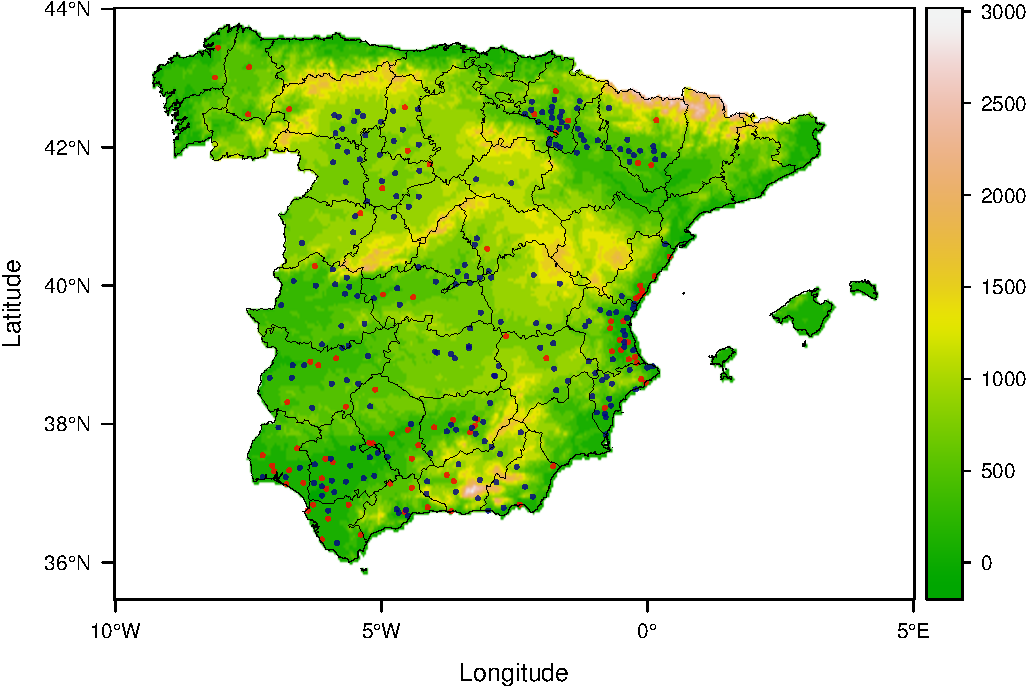
\includegraphics[width=\textwidth]{figs/mapaSIAR_crop}
  \caption{Meteorological stations of the SIAR network. The color key
    indicates the altitude (meters).}
  \label{fig:SIAR_map}
\end{figure}

\subsection{Daily Data of Different Meteorological Variables}
\label{sec:org1a1fd41}
As an example of multiple time series with different scales, we
will use 8 years (from January 2004 to December 2011) of daily
data corresponding to several meteorological variables measured at
the SIAR station located at Aranjuez (Madrid, Spain) available on
the SIAR webpage\footnote{\url{http://eportal.magrama.gob.es/websiar}}. The \texttt{aranjuez.gz} file, available in the
\texttt{data} folder of the book repository, contains this information
with several meteorological variables: average, maximum, and
minimum ambient temperature; average and maximum humidity; average
and maximum wind speed; rainfall; solar radiation on the
horizontal plane; and evotranspiration.

The \texttt{read.zoo} from the \texttt{zoo} package accepts this string and
downloads the data to construct a \texttt{zoo} object. Several
arguments are passed directly to \texttt{read.table} (\texttt{header}, \texttt{skip},
etc.) and are detailed conveniently on the help page of this
function. The \texttt{index.column} is the number of the column with the
time index, and \texttt{format} defines the date format of this index.

\index{Packages!zoo@\texttt{zoo}}
\index{read.zoo@\texttt{read.zoo}}

\lstset{language=r,label= ,caption= ,captionpos=b,numbers=none}
\begin{lstlisting}
library(zoo)
  
aranjuez <- read.zoo("data/aranjuez.gz",
                     index.column = 3, format = "%d/%m/%Y",
                     fileEncoding = 'UTF-16LE',
                     header = TRUE, fill = TRUE,
                     sep = ';', dec = ",", as.is = TRUE)
aranjuez <- aranjuez[, -c(1:4)]
  
names(aranjuez) <- c('TempAvg', 'TempMax', 'TempMin',
                     'HumidAvg', 'HumidMax',
                     'WindAvg', 'WindMax',
                     'Radiation', 'Rain', 'ET')
  
  
summary(aranjuez)
\end{lstlisting}

\begin{verbatim}
     Index               TempAvg          TempMax         TempMin       
 Min.   :2004-01-01   Min.   :-5.310   Min.   :-2.36   Min.   :-12.980  
 1st Qu.:2005-12-29   1st Qu.: 7.692   1st Qu.:14.53   1st Qu.:  1.520  
 Median :2008-01-09   Median :13.810   Median :21.67   Median :  7.170  
 Mean   :2008-01-03   Mean   :14.405   Mean   :22.54   Mean   :  6.894  
 3rd Qu.:2010-01-02   3rd Qu.:21.615   3rd Qu.:30.89   3rd Qu.: 12.590  
 Max.   :2011-12-31   Max.   :30.680   Max.   :41.91   Max.   : 22.710  
                                       NA's   :3       NA's   :7        
    HumidAvg        HumidMax         WindAvg         WindMax      
 Min.   :19.89   Min.   : 35.88   Min.   :0.250   Min.   : 1.550  
 1st Qu.:47.04   1st Qu.: 81.60   1st Qu.:0.670   1st Qu.: 3.840  
 Median :62.49   Median : 90.90   Median :0.920   Median : 5.150  
 Mean   :62.11   Mean   : 87.21   Mean   :1.166   Mean   : 5.467  
 3rd Qu.:77.30   3rd Qu.: 94.90   3rd Qu.:1.430   3rd Qu.: 6.760  
 Max.   :99.50   Max.   :103.00   Max.   :6.450   Max.   :18.060  
 NA's   :2       NA's   :10                                       
   Radiation          Rain              ET       
 Min.   : 0.28   Min.   : 0.000   Min.   :0.000  
 1st Qu.: 9.37   1st Qu.: 0.000   1st Qu.:1.160  
 Median :16.67   Median : 0.000   Median :2.750  
 Mean   :16.73   Mean   : 1.046   Mean   :3.088  
 3rd Qu.:24.63   3rd Qu.: 0.200   3rd Qu.:4.923  
 Max.   :32.74   Max.   :49.730   Max.   :8.560  
                                  NA's   :14
\end{verbatim}

\index{zoo@\texttt{zoo}}

From the summary it is clear that parts of these time series include erroneous outliers that can be
safely removed:
\lstset{language=r,label= ,caption= ,captionpos=b,numbers=none}
\begin{lstlisting}
aranjuezClean <- within(as.data.frame(aranjuez),{
    TempMin[TempMin>40] <- NA
    HumidMax[HumidMax>100] <- NA
    WindAvg[WindAvg>10] <- NA
    WindMax[WindMax>10] <- NA
})

aranjuez <- zoo(aranjuezClean, index(aranjuez))

summary(aranjuez)
\end{lstlisting}

\begin{verbatim}
     Index               TempAvg          TempMax         TempMin       
 Min.   :2004-01-01   Min.   :-5.310   Min.   :-2.36   Min.   :-12.980  
 1st Qu.:2005-12-29   1st Qu.: 7.692   1st Qu.:14.53   1st Qu.:  1.520  
 Median :2008-01-09   Median :13.810   Median :21.67   Median :  7.170  
 Mean   :2008-01-03   Mean   :14.405   Mean   :22.54   Mean   :  6.894  
 3rd Qu.:2010-01-02   3rd Qu.:21.615   3rd Qu.:30.89   3rd Qu.: 12.590  
 Max.   :2011-12-31   Max.   :30.680   Max.   :41.91   Max.   : 22.710  
                                       NA's   :3       NA's   :7        
    HumidAvg        HumidMax         WindAvg         WindMax      
 Min.   :19.89   Min.   : 35.88   Min.   :0.250   Min.   : 1.550  
 1st Qu.:47.04   1st Qu.: 81.60   1st Qu.:0.670   1st Qu.: 3.785  
 Median :62.49   Median : 90.90   Median :0.920   Median : 5.030  
 Mean   :62.11   Mean   : 87.20   Mean   :1.166   Mean   : 5.216  
 3rd Qu.:77.30   3rd Qu.: 94.90   3rd Qu.:1.430   3rd Qu.: 6.540  
 Max.   :99.50   Max.   :100.00   Max.   :6.450   Max.   :10.000  
 NA's   :2       NA's   :11                       NA's   :115     
   Radiation          Rain              ET       
 Min.   : 0.28   Min.   : 0.000   Min.   :0.000  
 1st Qu.: 9.37   1st Qu.: 0.000   1st Qu.:1.160  
 Median :16.67   Median : 0.000   Median :2.750  
 Mean   :16.73   Mean   : 1.046   Mean   :3.088  
 3rd Qu.:24.63   3rd Qu.: 0.200   3rd Qu.:4.923  
 Max.   :32.74   Max.   :49.730   Max.   :8.560  
                                  NA's   :14
\end{verbatim}


\subsection{Solar Radiation Measurements from Different Locations}
\label{sec:org3b3fba5}
As an example of multiple time series with the same scale, we will use
data of daily solar radiation measurements from different locations.

\index{Data!Solar radiation}
\index{Data!SIAR}

Daily solar radiation incident on the horizontal plane is registered
by meterological stations and estimated from satellite images. This
meteorological variable is important for a wide variety of scientific
disciplines and engineering applications. Its variations and trends,
dependent on the location (mainly latitude, and also longitude and
altitude) and on time (day of the year), have been analyzed and
modeled in a huge collection of papers and reports. In this section
we will focus our attention on the time evolution of the solar
radiation. The spatial distribution and the spatio-time behavior will
be the subject of later sections.

The stations of the SIAR network include first-class pyranometers
according to the World Meteorological Organization (WMO), whose
absolute accuracy is within \(\pm 5\%\) and is typically lower than \(\pm
3\%\). Solar irradiance is recorded every 15 minutes and then
collated through a datalogger within the station to generate the daily
irradiation, which is later sent to the regional and national centers.

The file \texttt{navarra.RData} contains daily solar radiation data of 2011
from the meteorological stations of Navarra, Spain. The names of the
dataset are the abbreviations of each station name.

\lstset{language=r,label= ,caption= ,captionpos=b,numbers=none}
\begin{lstlisting}
library(zoo)

load('data/navarra.RData')

summary(navarra)
\end{lstlisting}

\begin{verbatim}
     Index                 Arzr             Adó              Lmbr       
 Min.   :2011-01-01   Min.   : 1.562   Min.   : 0.028   Min.   : 2.122  
 1st Qu.:2011-04-02   1st Qu.: 8.680   1st Qu.: 7.630   1st Qu.: 8.610  
 Median :2011-07-02   Median :16.770   Median :15.680   Median :17.080  
 Mean   :2011-07-02   Mean   :16.627   Mean   :15.717   Mean   :16.767  
 3rd Qu.:2011-10-01   3rd Qu.:24.590   3rd Qu.:23.970   3rd Qu.:24.800  
 Max.   :2011-12-31   Max.   :32.400   Max.   :32.060   Max.   :32.820  
                                                                        
      Ancn             Artj            Aibr            SMdU       
 Min.   : 0.009   Min.   : 1.32   Min.   : 0.94   Min.   : 0.971  
 1st Qu.: 6.387   1st Qu.: 8.26   1st Qu.: 7.99   1st Qu.: 8.075  
 Median :13.950   Median :15.43   Median :16.08   Median :15.870  
 Mean   :15.140   Mean   :15.84   Mean   :16.21   Mean   :16.032  
 3rd Qu.:23.760   3rd Qu.:23.47   3rd Qu.:24.29   3rd Qu.:24.490  
 Max.   :34.630   Max.   :32.21   Max.   :32.54   Max.   :31.450  
 NA's   :4                                        NA's   :10      
      MrdA             Lern             Brgt             Olit       
 Min.   : 0.125   Min.   : 1.042   Min.   : 0.125   Min.   : 1.562  
 1st Qu.: 8.180   1st Qu.: 8.080   1st Qu.: 8.180   1st Qu.: 8.680  
 Median :15.760   Median :15.210   Median :15.760   Median :16.770  
 Mean   :15.584   Mean   :15.531   Mean   :15.584   Mean   :16.627  
 3rd Qu.:23.065   3rd Qu.:23.480   3rd Qu.:23.065   3rd Qu.:24.590  
 Max.   :31.210   Max.   :32.110   Max.   :31.210   Max.   :32.400  
 NA's   :2                         NA's   :2                        
      Flcs             Mrdf             Trbn             Srtg       
 Min.   : 1.061   Min.   : 1.424   Min.   : 0.051   Min.   : 1.398  
 1st Qu.: 8.080   1st Qu.: 8.685   1st Qu.: 8.467   1st Qu.: 8.998  
 Median :15.810   Median :16.980   Median :18.030   Median :16.475  
 Mean   :15.952   Mean   :16.892   Mean   :17.609   Mean   :16.329  
 3rd Qu.:23.570   3rd Qu.:24.608   3rd Qu.:26.065   3rd Qu.:23.348  
 Max.   :32.220   Max.   :31.950   Max.   :33.250   Max.   :31.210  
                  NA's   :13       NA's   :23       NA's   :27      
      BR.P             Funs             BR.B             Cdrt       
 Min.   : 1.039   Min.   : 1.051   Min.   : 1.327   Min.   : 1.438  
 1st Qu.: 8.140   1st Qu.: 8.830   1st Qu.: 8.790   1st Qu.: 8.100  
 Median :16.660   Median :16.360   Median :16.990   Median :15.770  
 Mean   :16.540   Mean   :16.493   Mean   :16.465   Mean   :15.719  
 3rd Qu.:24.590   3rd Qu.:24.970   3rd Qu.:24.400   3rd Qu.:23.390  
 Max.   :32.010   Max.   :32.610   Max.   :32.270   Max.   :31.170  
                                                                    
      Crll             Tudl             Fitr             Cscn       
 Min.   : 1.283   Min.   : 1.667   Min.   : 0.395   Min.   : 1.233  
 1st Qu.: 8.610   1st Qu.:10.043   1st Qu.: 7.850   1st Qu.: 8.140  
 Median :15.360   Median :17.375   Median :14.360   Median :15.080  
 Mean   :15.714   Mean   :17.453   Mean   :15.026   Mean   :15.751  
 3rd Qu.:23.100   3rd Qu.:25.317   3rd Qu.:22.950   3rd Qu.:23.640  
 Max.   :31.060   Max.   :30.880   Max.   :30.450   Max.   :32.130  
                  NA's   :163                                       
      Ablt            LsAr             Sesm       
 Min.   : 1.45   Min.   : 0.915   Min.   : 0.880  
 1st Qu.: 8.52   1st Qu.: 7.590   1st Qu.: 6.878  
 Median :15.51   Median :14.370   Median :13.230  
 Mean   :15.86   Mean   :15.044   Mean   :14.487  
 3rd Qu.:23.50   3rd Qu.:22.620   3rd Qu.:21.350  
 Max.   :31.05   Max.   :31.390   Max.   :31.280  
                                  NA's   :24
\end{verbatim}

\section{Unemployment in the United States}
\label{sec:org56131cd}
As an example of time series that can be displayed both in individual
and in aggregate, we will use the unemployment data in the United
States. The information on unemployed persons by industry and class of
worker is available in Table A-14 published by the Bureau of Labor
Statistics\footnote{\url{http://www.bls.gov/webapps/legacy/cpsatab14.htm}}.

The dataset arranges the information with a row for each category
(\texttt{Series.ID}) and a column for each monthly value. In addition, there
are columns with the annual summaries (\texttt{annualCols}). We rearrange
this \texttt{data.frame}, dropping the \texttt{Series.ID} and the annual columns,
and transpose the data.

\index{Data!Unemployment}

\lstset{language=r,label= ,caption= ,captionpos=b,numbers=none}
\begin{lstlisting}
unemployUSA <- read.csv('data/unemployUSA.csv')
nms <- unemployUSA$Series.ID
##columns of annual summaries
annualCols <- 14 + 13*(0:12)
## Transpose. Remove annual summaries
unemployUSA <- as.data.frame(t(unemployUSA[,-c(1, annualCols)]))
## First 7 characters can be suppressed
names(unemployUSA) <- substring(nms, 7)

summary(unemployUSA)
\end{lstlisting}

\begin{verbatim}
     32230            32231            32232            32235     
 Min.   :  2.00   Min.   : 384.0   Min.   : 596.0   Min.   : 701  
 1st Qu.: 22.00   1st Qu.: 626.8   1st Qu.: 774.2   1st Qu.:1019  
 Median : 30.00   Median : 823.0   Median :1024.0   Median :1176  
 Mean   : 37.76   Mean   : 981.0   Mean   :1091.4   Mean   :1303  
 3rd Qu.: 46.00   3rd Qu.:1190.2   3rd Qu.:1300.5   3rd Qu.:1707  
 Max.   :125.00   Max.   :2440.0   Max.   :2010.0   Max.   :2154  
 NA's   :6        NA's   :6        NA's   :6        NA's   :6     
     32236           32237           32238           32239       
 Min.   :129.0   Min.   : 77.0   Min.   :184.0   Min.   : 504.0  
 1st Qu.:226.0   1st Qu.:144.0   1st Qu.:268.0   1st Qu.: 743.0  
 Median :267.0   Median :194.5   Median :317.0   Median : 923.5  
 Mean   :315.7   Mean   :200.9   Mean   :375.2   Mean   :1014.2  
 3rd Qu.:420.2   3rd Qu.:244.8   3rd Qu.:508.8   3rd Qu.:1346.8  
 Max.   :657.0   Max.   :373.0   Max.   :717.0   Max.   :1785.0  
 NA's   :6       NA's   :6       NA's   :6       NA's   :6       
     32240            32241            32242           35109      
 Min.   : 293.0   Min.   : 636.0   Min.   :161.0   Min.   : 35.0  
 1st Qu.: 534.5   1st Qu.: 877.5   1st Qu.:265.0   1st Qu.:102.2  
 Median : 621.0   Median : 976.5   Median :313.5   Median :135.0  
 Mean   : 744.0   Mean   :1092.1   Mean   :351.6   Mean   :144.3  
 3rd Qu.: 994.8   3rd Qu.:1395.0   3rd Qu.:451.5   3rd Qu.:176.0  
 Max.   :1430.0   Max.   :1804.0   Max.   :618.0   Max.   :318.0  
 NA's   :6        NA's   :6        NA's   :6       NA's   :6      
     28615            35181      
 Min.   : 269.0   Min.   :178.0  
 1st Qu.: 458.0   1st Qu.:260.5  
 Median : 543.5   Median :311.5  
 Mean   : 619.9   Mean   :371.8  
 3rd Qu.: 748.8   3rd Qu.:523.8  
 Max.   :1349.0   Max.   :730.0  
 NA's   :6        NA's   :6
\end{verbatim}

With the transpose, the column names of the original data set are
now the row names of the \texttt{data.frame}. The \texttt{as.yearmon} function
of the \texttt{zoo} package converts the character vector of names into a
\texttt{yearmon} vector, a class for representing monthly data. With
\texttt{Sys.setlocale("LC\_TIME", 'C')} we ensure that month abbreviations
(\texttt{\%b}) are correctly interpreted in a non-English locale. This
vector is the time index of a new \texttt{zoo} object. 

\index{Packages!zoo@\texttt{zoo}}
\index{as.yearmon@\texttt{as.yearmon}}
\index{apply@\texttt{apply}}
\index{zoo@\texttt{zoo}}

\lstset{language=r,label= ,caption= ,captionpos=b,numbers=none}
\begin{lstlisting}
library(zoo)
  
Sys.setlocale("LC_TIME", 'C')
idx <- as.yearmon(row.names(unemployUSA), format='%b.%Y')
unemployUSA <- zoo(unemployUSA, idx)
\end{lstlisting}


Finally, those rows with \texttt{NA} values are removed.

\lstset{language=r,label= ,caption= ,captionpos=b,numbers=none}
\begin{lstlisting}
isNA <- apply(is.na(unemployUSA), 1, any)
unemployUSA <- unemployUSA[!isNA,]

summary(unemployUSA)
\end{lstlisting}

\begin{verbatim}
     Index          32230            32231            32232       
 Min.   :2000   Min.   :  2.00   Min.   : 384.0   Min.   : 596.0  
 1st Qu.:2003   1st Qu.: 22.00   1st Qu.: 626.8   1st Qu.: 774.2  
 Median :2006   Median : 30.00   Median : 823.0   Median :1024.0  
 Mean   :2006   Mean   : 37.76   Mean   : 981.0   Mean   :1091.4  
 3rd Qu.:2009   3rd Qu.: 46.00   3rd Qu.:1190.2   3rd Qu.:1300.5  
 Max.   :2012   Max.   :125.00   Max.   :2440.0   Max.   :2010.0  
     32235          32236           32237           32238      
 Min.   : 701   Min.   :129.0   Min.   : 77.0   Min.   :184.0  
 1st Qu.:1019   1st Qu.:226.0   1st Qu.:144.0   1st Qu.:268.0  
 Median :1176   Median :267.0   Median :194.5   Median :317.0  
 Mean   :1303   Mean   :315.7   Mean   :200.9   Mean   :375.2  
 3rd Qu.:1707   3rd Qu.:420.2   3rd Qu.:244.8   3rd Qu.:508.8  
 Max.   :2154   Max.   :657.0   Max.   :373.0   Max.   :717.0  
     32239            32240            32241            32242      
 Min.   : 504.0   Min.   : 293.0   Min.   : 636.0   Min.   :161.0  
 1st Qu.: 743.0   1st Qu.: 534.5   1st Qu.: 877.5   1st Qu.:265.0  
 Median : 923.5   Median : 621.0   Median : 976.5   Median :313.5  
 Mean   :1014.2   Mean   : 744.0   Mean   :1092.1   Mean   :351.6  
 3rd Qu.:1346.8   3rd Qu.: 994.8   3rd Qu.:1395.0   3rd Qu.:451.5  
 Max.   :1785.0   Max.   :1430.0   Max.   :1804.0   Max.   :618.0  
     35109           28615            35181      
 Min.   : 35.0   Min.   : 269.0   Min.   :178.0  
 1st Qu.:102.2   1st Qu.: 458.0   1st Qu.:260.5  
 Median :135.0   Median : 543.5   Median :311.5  
 Mean   :144.3   Mean   : 619.9   Mean   :371.8  
 3rd Qu.:176.0   3rd Qu.: 748.8   3rd Qu.:523.8  
 Max.   :318.0   Max.   :1349.0   Max.   :730.0
\end{verbatim}

\section{Gross National Income and CO\(_{\text{2}}\) Emissions}
\label{sec:org9ba3273}
The catalog data of the World Bank Open Data initiative includes the
World Development Indicators (WDI)\footnote{\url{http://databank.worldbank.org/data/reports.aspx?source=world-development-indicators}}. Among them we will analyze
the evolution of the relationship between Gross National Income (GNI)
and \(CO_2\) emissions for a set of countries. The package \texttt{WDI} is able
to search and download these data series.

\index{Data!World Bank}
\index{Data!CO2@$CO_2$}
\index{Data!GNI}
\index{Packages!WDI@\texttt{WDI}}

\lstset{language=r,label= ,caption= ,captionpos=b,numbers=none}
\begin{lstlisting}
library(WDI)
    
CO2data <- WDI(indicator=c('EN.ATM.CO2E.PC', 'EN.ATM.CO2E.PP.GD',
                           'NY.GNP.MKTP.PP.CD', 'NY.GNP.PCAP.PP.CD'),
               start=2000, end=2011,
               country=c('BR', 'CN', 'DE', 'ES',
                         'FI', 'FR', 'GR', 'IN', 'NO', 'US'))

names(CO2data) <- c('iso2c', 'Country.Name', 'Year',
                    'CO2.capita', 'CO2.PPP',
                    'GNI.PPP', 'GNI.capita')

summary(CO2data)
\end{lstlisting}

\begin{verbatim}
    iso2c           Country.Name            Year        CO2.capita     
 Length:120         Length:120         Min.   :2000   Min.   : 0.9674  
 Class :character   Class :character   1st Qu.:2003   1st Qu.: 4.8660  
 Mode  :character   Mode  :character   Median :2006   Median : 7.9145  
                                       Mean   :2006   Mean   : 7.9130  
                                       3rd Qu.:2008   3rd Qu.: 9.9587  
                                       Max.   :2011   Max.   :20.1788  
    CO2.PPP          GNI.PPP            GNI.capita   
 Min.   :0.1356   Min.   :1.375e+11   Min.   : 1960  
 1st Qu.:0.2120   1st Qu.:3.036e+11   1st Qu.:10978  
 Median :0.3037   Median :2.014e+12   Median :28730  
 Mean   :0.3440   Mean   :3.349e+12   Mean   :26753  
 3rd Qu.:0.3963   3rd Qu.:3.540e+12   3rd Qu.:37872  
 Max.   :0.9194   Max.   :1.580e+13   Max.   :62640
\end{verbatim}


Only two minor modifications are needed: Remove the missing values and
convert the \texttt{Country.Name} column into a \texttt{factor}. This first
modification will save problems when displaying the time series, and
the \texttt{factor} conversion will be useful for grouping.

\lstset{language=r,label= ,caption= ,captionpos=b,numbers=none}
\begin{lstlisting}
isNA <- apply(is.na(CO2data), 1, any)
CO2data <- CO2data[!isNA, ]

CO2data$Country.Name <- factor(CO2data$Country.Name)

summary(CO2data)
\end{lstlisting}

\begin{verbatim}
    iso2c            Country.Name      Year        CO2.capita     
 Length:120         Brazil :12    Min.   :2000   Min.   : 0.9674  
 Class :character   China  :12    1st Qu.:2003   1st Qu.: 4.8660  
 Mode  :character   Finland:12    Median :2006   Median : 7.9145  
                    France :12    Mean   :2006   Mean   : 7.9130  
                    Germany:12    3rd Qu.:2008   3rd Qu.: 9.9587  
                    Greece :12    Max.   :2011   Max.   :20.1788  
                    (Other):48                                    
    CO2.PPP          GNI.PPP            GNI.capita   
 Min.   :0.1356   Min.   :1.375e+11   Min.   : 1960  
 1st Qu.:0.2120   1st Qu.:3.036e+11   1st Qu.:10978  
 Median :0.3037   Median :2.014e+12   Median :28730  
 Mean   :0.3440   Mean   :3.349e+12   Mean   :26753  
 3rd Qu.:0.3963   3rd Qu.:3.540e+12   3rd Qu.:37872  
 Max.   :0.9194   Max.   :1.580e+13   Max.   :62640
\end{verbatim}
